\chapter{Background}
\label{ch:background}

The foundations of the thesis are established in this chapter. A top-down approach is followed. The first topic treated is the mathematical theory of the finite element method. How this theory is translated into software is subsequently discussed; in particular, a revolutionary approach based upon automated code generation is explored. The core libraries that make this approach possible are surveyed. The state of the art in performance optimization is then reviewed, with emphasis on the fundamental class of loop reordering transformations. An overview of the successful domain-specific abstractions that have inspired some of the core contributions of this thesis concludes the chapter. Some of the relevant related work is introduced, although extended literature review is provided in the later chapters.


\section{The Finite Element Method}
\label{sec:bkg:fem}
Computational methods based upon finite elements are used to approximate the solution of partial differential equations (henceforth, PDEs) in a wide variety of domains. The mathematical abstraction used in the finite element method is extremely powerful: not only does it help reasoning about the problem, but also provides systematic ways of deriving effective computer implementations. This, however, has a price in terms of complexity. Here, we limit ourselves to reviewing the aspects that are essential for understanding the contributions in Chapters~\ref{ch:optimality} and~\ref{ch:lowlevelopt}. The content and the notation used in this section are inspired by~\cite{florian-thesis},~\cite{Fenics} and~\cite{quadrature-olegaard}. For a complete treatment of the subject, the reader is invited to refer to~\cite{brenner-and-scott}.



\subsection{Weak Formulation}
\label{sec:bkg:var-problems}
In a {\em boundary value problem}, the solution of a (partial) differential equation subject to a set of {\em boundary conditions} is sought. The boundary conditions specify the behaviour of the unknown at the domain boundary. 

We introduce two spaces of functions, $U$ and $V$, called respectively trial space and test space. These function spaces may have desirable properties, such as differentiability. We consider the {\em variational} or {\em weak} formulation of a linear boundary value problem\footnote{Non-linear problems require refinements that are out of the scope of this review.}

\begin{equation}
\label{sec:bkg:eq:strong}
\text{Find}\ u \in U\ \text{such that}\ \ \ \ a(u, v) = L(v)\ \ \ \ \forall v \in V
\end{equation}

where $u$ is the sought problem solution. In this formulation, $a$ is a bilinear form (a map $U \times V \rightarrow \mathbb{R}$, linear in each argument separately) and $L$ is a linear form (a linear map $V \rightarrow \mathbb{R}$). The term ``variational'' stems from the fact that the test function $v$ can vary arbitrarily. The reader unfamiliar with the theory of Hilbert spaces may find this formulation unusual. The underlying idea of the variational formulation consists of ``transferring'' certain requirements on the unknown (e.g., differentiability) to $v$. 
%A deep understanding of meaning and implications of a weak formulation goes, however, far beyond the objectives of this section.

In the finite element method, the variational problem is discretized by using {\it discrete} trial and test spaces, namely $U_h \subset U$ and $V_h \subset V$. This leads to restating~(\ref{sec:bkg:eq:strong}) as

\begin{equation}
\label{sec:bkg:eq:disc-var}
\text{Find}\ u_h \in U_h \subset U\ \text{such that}\ \ \ \ a(u_h, v_h) = L(v_h)\ \ \ \ \forall v_h \in V_h \subset V
\end{equation}

Let $\lbrace \psi_j \rbrace_{j=1}^N$ be a set of basis functions spanning $U_h$ and let $\lbrace \phi_i \rbrace_{i=1}^{N}$ be a set of basis functions spanning $V_h$. The unknown solution $u$ can be approximated as a linear combination of the basis functions $\lbrace \psi_j \rbrace_{j=1}^N$,

\begin{equation}
u_h = \sum_{j=1}^N \hat{u}_j \psi_j.
\end{equation}

The equation in (\ref{sec:bkg:eq:disc-var}) can then be reformulated as:

\begin{equation}
\sum_{j=1}^N \hat{u}_j \, a(\psi_j, \phi_i) = L(\phi_i),\ \ \ i=1,2,...,N
\end{equation}

From the solution of the linear system

\begin{equation}
\label{sec:bkg:eq:lin-sys}
Au = b
\end{equation}

where

\begin{equation}
\label{sec:bkg:eq:disc-op}
\centering
\begin{split}
A_{ij} = a(\psi_j,\phi_i) \\
b_i = L(\phi_i)
\end{split}
\end{equation}

we determine the set of {\em degrees of freedom} $U$ to express $u_h$. The matrix $A$ and the vector $b$ can be seen as the discrete operators arising from the bilinear form $a$ and from the linear form $L$ for the given choice of basis functions.

The underlying assumption of this formulation is that the finite dimensional subspaces $U_h$ and $V_h$ can be constructed. As elaborated in Section~\ref{sec:bkg:finite-elements}, $U_h$ and $V_h$ are constructed by decomposing the PDE domain into a set of {\em finite elements} and by combining the local function spaces defined on these elements. 



\subsection{Local and Global Function Spaces}
\label{sec:bkg:finite-elements}
In the finite element method, the domain $\Omega$ of the PDE is partitioned into a finite set of disjoint cells $\lbrace K \rbrace$; that is, $\bigcup K = \Omega$ and $\bigcap K = \emptyset$. This forms a {\em mesh}. 

\paragraph{Finite elements}
As originally formalized in~\cite{ciarlet-fem}, a finite element is a triple $\langle K,\mathcal{P}_K,\mathcal{L}_K \rangle$, where:
\begin{itemize}
\item $K$ is a cell in the mesh with non-empty interior and piecewise smooth boundary;
\item $\mathcal{P}_K$ is a finite dimensional ``local'' function space of dimension $n_K$;
\item the set of degrees of freedom (nodes) $\mathcal{L}_K$ is a basis $\lbrace l_1^K, l_2^K, ..., l_{n_K}^K\rbrace$ for $\mathcal{P}'_K$, the dual space of $\mathcal{P}_K$. 
\end{itemize}
This definition allows imposing constraints on the set of basis functions $\lbrace \phi_1^K, \phi_2^K, ..., \phi_{n_K}^K\rbrace$ spanning $\mathcal{P}_K$. For instance, to enforce a {\em nodal basis} for $\mathcal{P}_K$ -- a particularly useful property for expressing solutions in $U_h$ -- we can impose that the relationship

\begin{equation}
l_i^K(\phi_j^K) = \delta_{ij},\ \ \ \ i,j = 1,2,...,n_K
\end{equation}

where $\delta_{ij}$ is the Kronecker delta, must be satisfied. This allows the expression of any $v \in \mathcal{P}_K$ as

\begin{equation}
v = \sum_{i=1}^{n_K} l_i^K(v) \, \phi_i^K.
\end{equation}

Each linear functional in $\mathcal{L}_K$ is used to evaluate one degree of freedom of $v$ in terms of the chosen nodal basis. In other words, we can refer to both the coefficients $U$ introduced in the previous section and $\mathcal{L}_K$ as the degrees of freedom.

\paragraph{Example: the triangular degree 1 Lagrange element}
The following example is extracted from~\cite{Fenics}. Consider a triangular cell $K$ and let $\mathcal{P}_K$ be the space of polynomials of order $1$ on $K$. Let $\mathcal{L}_K$ be the set of bounded linear functionals representing point evaluation at the vertices $\boldsymbol{x}^i$ ($i=1,2,3$) of $K$ such that

\begin{equation}
\centering
\begin{split}
l_i^K : \mathcal{P^K} \rightarrow \mathbb{R} \\
l_i^K(v) = v(\boldsymbol{x}^i)
\end{split}
\end{equation}

Since if $v$ is zero at each vertex then $v$ must be zero everywhere, $\mathcal{L}_K$ really is a basis for $\mathcal{P}'_K$, so what we have defined is indeed a finite element. In particular, if we take $\boldsymbol{x}^1 = (0, 0),\ \boldsymbol{x}^2 = (1,0),\ \boldsymbol{x}^3 = (0,1)$, we have that the nodal basis is given by:

\begin{equation}
\phi_1(\boldsymbol{x}) = 1 - x_1 - x_2,\ \ \ \ \ \phi_2(\boldsymbol{x}) = x_1,\ \ \ \ \ \phi_3(\boldsymbol{x}) = x_2.
\end{equation}

\paragraph{Construction of the global function spaces}
A {\em local-to-global mapping} allows to patch together the finite elements to form a global function space, for instance the set of trial functions $U_h = \operatorname{span}\lbrace \psi_j \rbrace_{j=1}^N$ introduced in Section~\ref{sec:bkg:var-problems}. A local-to-global mapping is a function

\begin{equation}
\iota_K : [1,n_K] \rightarrow [1,N]
\end{equation}

that maps the local degrees of freedom $\mathcal{L}_K$ to global degrees of freedom $\mathcal{L}$. The mappings $\iota_K$, together with the choice of $\mathcal{L}_K$, determine the continuity of a function space or, in simpler words, the continuity of a function throughout the domain $\Omega$. The reader is invited to refer to~\cite{Fenics} for a comprehensive description of this step.

\subsection{The Reference Element}
\label{sec:bkg:refel}
One of the central aspects of the finite element method is that global function spaces are often defined in terms of a {\em reference finite element} ${<}\hat{K}, \hat{\mathcal{P}}, \hat{\mathcal{L}}{>}$ and a set of invertible mappings $\lbrace \mathcal{G}_K\rbrace_{K}$ from $\hat{K}$ to each cell in the mesh such that $K = \mathcal{G}_K(\hat{K})$.  This situation is illustrated in Figure~\ref{fig:bkg:reference-el}.

\begin{figure}
\begin{CenteredBox}
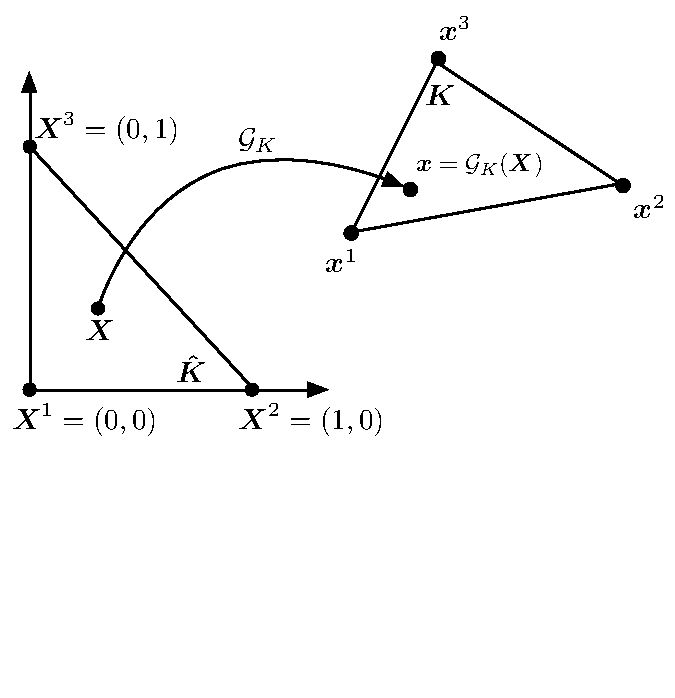
\includegraphics[scale=0.8]{background/figures/reference-element}
\end{CenteredBox}
\caption{Affine mapping from the reference element $\hat{K}$ to an element $K$.}
\label{fig:bkg:reference-el}
\end{figure}

For each $K$, $\mathcal{G}_K$ also allows to generate $\mathcal{P}_K$ and $\mathcal{L}_K$.  The complexity of this process depends on the mapping itself. In the simplest case, the mapping is affine; that is, expressible as $\mathcal{G}_K(\hat{\boldsymbol{x}}) = M_K \hat{\boldsymbol{x}} + w_K$, where $M_K$ and $w_K$ are, respectively, some matrix and vector.


\subsection{Assembly}
\label{sec:bkg:assembly}
The {\em assembly} is the phase in which the matrix $A$ and the vector $b$ in (\ref{sec:bkg:eq:disc-op}) are constructed. This is accomplished by adding the contributions from each $K$ to $A$ and $b$. Let us consider the bilinear form $a$. Since the operator is linear, we can express $a$ as

\begin{equation}
a = \sum_{K} a_K
\end{equation}

where $a_K$ is an element bilinear form. We can then define the local element matrix

\begin{equation}
A_i^K = a_K (\psi_{i_1}^K, \phi_{i_2}^K)
\end{equation}

where $i \in \mathcal{I}_K$, the index set on $A_i^K$. That is, $\mathcal{I}_K = \lbrace (1,1), ..., (n_U, n_V) \rbrace$, with $n_U$ and $n_V$ representing the number of degrees of freedom for the local trial functions $\psi^K \in U_h^K$ and the local test functions $\phi^K \in V_h^K$. The element matrix $A^K$ is therefore a (typically dense) matrix of dimension $n_U \times n_V$.

Now let $\iota_K^U$ and $\iota_K^V$ be the local-to-global mappings for the local discrete function spaces $U_h^K$ and $V_h^K$. We can define, for each $K$, the collective local-to-global mapping $\iota_K : \mathcal{I}_K \rightarrow \mathcal{I}$ such that

\begin{equation}
\iota_K (i) = (\iota_K^U(i_1), \iota_K^V(i_2)),\ \ \ \forall i \in \mathcal{I}_K.
\end{equation}

This simply maps a pair of local degrees of freedom to a pair of global degrees of freedom. Let $\mathcal{T}$ be the subset of the cells in the mesh in which $\psi_{i_1}$ and $\phi_{i_2}$ are both non-zero. Note that here we are considering the global functions whose restrictions to $K$ gives $\psi_{i_1}^K$ and $\phi_{i_2}^K$. By construction, $\iota_K$ is invertible if $K \in \mathcal{T}$. At this point, we have all the ingredients to formulate the computation of $A$ as the sum of local contributions from the elements in the mesh:

\begin{equation}
\begin{split}
A_i & = \sum_{K \in \mathcal{T}} a_K (\psi_{i_1},\phi_{i_2}) \\
& = \sum_{K \in \mathcal{T}} a_K(\psi_{(\iota_K^U)^{-1}(i_1)}^K, \phi_{(\iota_K^V)^{-1}(i_2)}^K) = \sum_{K \in \mathcal{T}} A_{\iota_K^{-1}(i)}^K
\end{split}
\end{equation} 

Similar conclusions may be drawn for the linear form $L$. We observe that this computation can be implemented as a single iteration over all cells in the mesh. On each cell, $A^K$ is computed and added to $A$ using the corresponding inverse map. This approach is particularly efficient because it only evaluates the non-zero entries in the sparse matrix $A$. More trivial implementations are possible, although they are rarely used in practice because of the higher computational cost.

We conclude with a clarification concerning the terminology. The assembly process is often described as a two-step procedure: {\em local assembly}  and {\em global assembly}. The former consists of computing the contributions of each element (i.e., the element matrices $A^K$); the latter represents the ``coupling'' of all $A^K$ into $A$. As we shall see, one of the main subjects of this thesis is the computational optimization of the local assembly phase.

\subsection{Local Assembly Example: from Math to Code}
\label{sec:bkg:math-to-code}
Because of its relevance in this thesis, we illustrate local assembly in a concrete example, the evaluation of the element matrix for a Laplacian operator. 

\subsubsection{Specification of the Laplacian operator}
Consider the weighted Laplace equation

\begin{equation}
- \nabla \cdot (w \nabla u) = 0
\end{equation}

in which $u$ is unknown, while $w$ is prescribed. The bilinear form associated with the weak variational form of the equation is:

\begin{equation}
\label{sec:bkg:eq:spec-laplacian}
a(v, u) = \int_\Omega w \nabla v \cdot \nabla u\ \mathrm{d}x
\end{equation}

The domain $\Omega$ of the equation is partitioned into a set of cells (elements) $T$ such that $\bigcup T = \Omega$ and $\bigcap T = \emptyset$. Assuming for simplicity that the sets of trial and test functions are the same and by defining $\lbrace \phi_i^K \rbrace$ as the set of local basis functions spanning $U$ and $V$ on the element $K$, we can express the local element matrix as

\begin{equation}
\label{sec:bkg:stiffness}
A_{ij}^K = \int_K w \nabla \phi_i^K \cdot \nabla \phi_j^K\ \mathrm{d}x
\end{equation}

The element vector $L$ can be determined in an analogous way. 

\subsubsection{Monomials}
\label{sec:bkg:monomials}
In this example, the element tensor is expressed as a single integral over the cell domain. In general, it is expressed as a sum of integrals over $K$, each integral being the product of derivatives of functions from sets of discrete spaces and, possibly, functions of some spatially varying coefficients. We refer to such integrals as the \textit{monomials} of the form. 

\subsubsection{Assembly with Quadrature}
$A_{ij}^K$ is numerically evaluated by means of a quadrature scheme. A quadrature scheme approximates an integral by evaluating the integrand at a set of {\em quadrature points}, each point multiplied with some suitable {\em quadrature weight}, and summing these values. By mapping the computation to a reference element as explained in Section~\ref{sec:bkg:refel} and by using the assembly procedure detailed in Section~\ref{sec:bkg:assembly}, a quadrature scheme for the Laplacian operator on $K$ is as follows

\begin{equation}
\begin{split}
A_{ij}^K & = \int_K w \nabla \phi_i^K \cdot \nabla \phi_j^K \\
& \approx w \sum_{k=1}^{N_q} W_k \nabla \phi_i^K(\boldsymbol{x}^k) \cdot \nabla \phi_j^K (\boldsymbol{x}^k) | \operatorname{det} \mathcal{G}_K'(\boldsymbol{x}^k) |,
\end{split}
\end{equation} 

where $\lbrace \boldsymbol{x}^1, \boldsymbol{x}^2, ..., \boldsymbol{x}^{N_q} \rbrace$ is the set of $N_q$ quadrature points, and $\lbrace W_1, W_2, ..., W_{N_q} \rbrace$ the corresponding set of quadrature weights scaled such that $\sum_{k=1}^{N_q} W_k = |\hat{K}|$. 

To compute a local basis function $\phi_i^K$ from a reference element basis function $\Phi_i$ we exploit the inverse map $\mathcal{G}_K^{-1}$, which allows us to write $\phi_i^K$ as $\phi_i^K = \Phi_i \circ \mathcal{G}_K^{-1}$. To evaluate the gradient of a basis function $\phi_i^K$ at a quadrature point $\boldsymbol{x}^k$, with $\boldsymbol{x}^k = \mathcal{G}_K(\boldsymbol{X}^k)$ and $\boldsymbol{X}^k \in \hat{K}$, we therefore have to compute a matrix-vector product

\begin{equation}
\nabla_x \phi_i^K(\boldsymbol{x}^k) = ((\mathcal{G}_K')^{-1})^{T}(\boldsymbol{x}^k) \nabla_X \Phi_i(\boldsymbol{X}^k).
\end{equation}

The term $(\mathcal{G}_K')^{-1}$ represents the inverse of the Jacobian matrix originating from the change of coordinates. The resulting scalar-valued expression for each entry $A_{ij}^K$, assuming $\Omega$ to be a domain of dimension $d$, reads as:

\begin{equation}
\label{eq:quadrature}
A_{ij}^K = \sum_{k=1}^{N_q} \sum_{\alpha_3=1}^n \phi_{\alpha_3}(\boldsymbol{X}^k) w_{\alpha_3} \sum_{\alpha_1=1}^d \sum_{\alpha_2=1}^d \sum_{\beta=1}^d \frac{\partial X_{\alpha_1}}{\partial x_{\beta}} \frac{\partial \phi_i^K(\boldsymbol{X}^k)}{\partial X_{\alpha_1}} \frac{\partial X_{\alpha_2}}{\partial x_{\beta}} \frac{\partial \phi_j^K(\boldsymbol{X}^k)}{\partial X_{\alpha_2}} \operatorname{det} \mathcal{G}_K' W^k.
\end{equation}


\subsubsection{Assembly with Tensor Contraction}
%\label{sec:tc}
Consider the case in which $\mathcal{G}_K : \hat{K} \rightarrow K$ is an affine mapping. Exploiting linearity, associativity and distributivity of the involved mathematical operators, we can rewrite (\ref{eq:quadrature}) as

\begin{equation}
\label{eq:tensor}
A_{ij}^K = \sum_{\alpha_1=1}^d \sum_{\alpha_2=1}^d \sum_{\alpha_3=1}^n \operatorname{det} \mathcal{G}_K' w_{\alpha_3} \sum_{\beta=1}^d \frac{\partial X_{\alpha_1}}{\partial x_{\beta}} \frac{\partial X_{\alpha_2}}{\partial x_{\beta}} \int_{K_0} \phi_{\alpha_3} \frac{\partial \phi_{i}}{\partial X_{\alpha_1}} \frac{\partial \phi_{j}}{\partial X_{\alpha_2}} dX.
\end{equation}

A generalization of this transformation has been proposed in~\cite{FFC-TC}. By only involving reference element terms, the integral in the equation can be pre-evaluated and stored in temporary variables. The evaluation of the local tensor can then be abstracted as

\begin{equation}
A_{ij}^K = \sum_{\alpha} A_{i j \alpha}^0 G_{K}^\alpha
\end{equation}

in which the pre-evaluated ``reference tensor'' $A_{i j \alpha}$ and the cell-dependent ``geometry tensor'' $G_{K}^\alpha$

\begin{equation}
A_{i j \alpha}^0 = \int_{K_0} \phi_{\alpha_3} \frac{\partial \phi_{i}}{\partial X_{\alpha_1}} \frac{\partial \phi_{j}}{\partial X_{\alpha_2}} dX,
\end{equation}

\begin{equation}
G_{K}^\alpha = \operatorname{det} \mathcal{G}_K' w_{\alpha_3} \sum_{\beta=1}^d \frac{\partial X_{\alpha_1}}{\partial x_{\beta}} \frac{\partial X_{\alpha_2}}{\partial x_{\beta}}
\end{equation}

are exposed.


\subsubsection{Qualitative Comparison of Quadrature and Tensor Contraction}
%\label{sec:qualitative}
Depending on form and discretization, the relative performance of the two approaches can vary quite dramatically. The presence of derivatives or coefficient functions in the input form increases the rank of the geometry tensor, which makes the traditional quadrature mode preferable for ``complex'' forms, due to a lower operation count. On the other hand, the tensor contraction mode leads to significant speed-ups in a wide class of ``simple'' forms, in which the geometry tensor remains sufficiently small. The discretization, particularly the relative polynomial order of trial, test, and coefficient functions, also plays a key role in the resulting operation count. 

\subsubsection{Towards a new Algorithm for Local Assembly}
The quadrature and tensor contraction modes have been implemented in the FEniCS Form Compiler~\citep{FFC-TC}, which we review in later sections. In this compiler, a heuristic is used to choose the most suitable mode for a given form. It consists of analysing each monomial in the form, counting the number of derivatives and coefficient functions, and checking if this number is greater than a constant found empirically \citep{Fenics}. In Chapter~\ref{ch:optimality}, {\em a novel algorithm} that goes beyond the dichotomy between quadrature and tensor contraction modes will be introduced. 


\subsubsection{Code Examples}
\label{sec:bkg:mathcode}

\begin{algorithm}[h]
\scriptsize\ttfamily
\SetAlgorithmName{LISTING}{}

\KwSty{void} weighted$\_$laplace(\KwSty{double} A[3][3], \KwSty{double} **coords, \KwSty{double} w[3]) \\
$\lbrace$ \\
~~// Compute Jacobian \\
~~\KwSty{double} J[4]; \\
~~compute$\_$jacobian$\_$triangle$\_$2d(J, coords); \\
~~\\
~~// Compute Jacobian inverse and determinant \\
~~\KwSty{double} K[4]; \\
~~\KwSty{double} detJ; \\
~~compute$\_$jacobian$\_$inverse$\_$triangle$\_$2d(K, detJ, J); \\
~~\KwSty{const double} det = fabs(detJ); \\
~~\\
~~// Quadrature weights \\
~~\KwSty{static const double} W[6] = {0.5}; \\
~~\\
~~// Basis functions \\
~~\KwSty{static const double} B[6][3] = $\lbrace\lbrace$...$\rbrace\rbrace$ ;\\
~~\KwSty{static const double} C[6][3] = $\lbrace\lbrace$...$\rbrace\rbrace$ ;\\
~~\KwSty{static const double} D[6][3] = $\lbrace\lbrace$...$\rbrace\rbrace$ ;\\
~~\\
~~\KwSty{for} (\KwSty{int} i = 0; i < 6; ++i) $\lbrace$ \\
~~~~\KwSty{double} f0  = 0.0;\\
~~~~\KwSty{for} (\KwSty{int} r  = 0; r < 3; ++r) $\lbrace$ \\
~~~~~~f0 += (w[r] * C[i][r]);\\
~~~~$\rbrace$ \\
~~~~\KwSty{for} (\KwSty{int} j = 0; j < 3; ++j) $\lbrace$\\
~~~~~~\KwSty{for} (\KwSty{int} k = 0; k < 3; ++k) $\lbrace$\\
~~~~~~~~A[j][k] += (((((K[1]*B[i][k]) + (K[3]*D[i][k])) * \\
~~~~~~~~~~~~~~~~~~~~~~((K[1]*B[i][j]) + (K[3]*D[i][j]))) + \\
~~~~~~~~~~~~~~~~~~~~~(((K[0]*B[i][k]) + (K[2]*D[i][k])) * \\
~~~~~~~~~~~~~~~~~~~~~~((K[0]*B[i][j]) + (K[2]*D[i][j]))))*det*W[i]*f0);\\
~~~~~~$\rbrace$\\
~~~~$\rbrace$\\
~~$\rbrace$\\
$\rbrace$
\caption{A possible implementation of Equation~\ref{eq:quadrature} assuming a 2D triangular mesh and polynomial order $1$ Lagrange basis functions.}
\label{code:weighted-laplace}
\end{algorithm}



A possible C implementation of (\ref{eq:quadrature}) is illustrated in Listing~\ref{code:weighted-laplace}. We assume a domain of dimension $d=2$ and polynomial order $1$ Lagrange elements. The values at the quadrature points of the derivatives of the basis functions are pre-tabulated in the \texttt{B} and \texttt{D} arrays (representing, respectively, the derivatives with respect to the coordinates $x$ and $y$). The values at the quadrature points of the basis functions spanning the field $w$ are pre-tabulated in the array \texttt{C}. Pre-tabulation, which is made possible by mapping the computation to a reference element, is fundamental to speed up the local assembly phase. The summation over the $N_q = 6$ quadrature points is implemented by the \texttt{i} loop. The summation over $\alpha_3$ for expressing $w$ is implemented by the loop \texttt{r}. The summations over the spatial dimensions $\alpha_1$, $\alpha_2$ and $\beta$ have been expanded in the ``assembly expression'' that evaluates the local element matrix $A$. The $K$ array includes the four components of the inverse of the Jacobian matrix for the change of coordinates. 

\begin{algorithm}[thpb]
\scriptsize\ttfamily
\SetAlgorithmName{LISTING}{}

\KwSty{void} burgers(\KwSty{double} A[12][12], \KwSty{double} **coords, \KwSty{double} **w) \\
$\lbrace$ \\
~~// Compute Jacobian \\
~~\KwSty{double} J[9]; \\
~~compute$\_$jacobian$\_$triangle$\_$3d(J, coords); \\
~~\\
~~// Compute Jacobian inverse and determinant \\
~~\KwSty{double} K[9]; \\
~~\KwSty{double} detJ; \\
~~compute$\_$jacobian$\_$inverse$\_$triangle$\_$3d(K, detJ, J); \\
~~\KwSty{const double} det = fabs(detJ); \\
~~\\
~~// Quadrature weights \\
~~\KwSty{static const double} W[5] = $\lbrace$...$\rbrace$\\
~~\\
~~// Basis functions \\
~~\KwSty{static const double} B[5][12] = $\lbrace\lbrace$...$\rbrace\rbrace$\\
~~\KwSty{static const double} C[5][12] = $\lbrace\lbrace$...$\rbrace\rbrace$\\
~~//11 other basis functions definitions \\
~~...\\
~~\KwSty{for} (\KwSty{int} i = 0; i$<$5; i++) $\lbrace$\\
~~~~\KwSty{double} f0 = 0.0;\\
~~~~//10 other declarations (f1, f2,...)\\
~~~~...\\
~~~~\KwSty{for} (\KwSty{int} r = 0; r$<$12; r++) $\lbrace$\\
~~~~~~f0 += (w[r][0]*C[i][r]);\\
~~~~~~//10 analogous statements (f1, f2, ...)\\
~~~~~~\\
~~~~$\rbrace$\\
~~~~\KwSty{for} (\KwSty{int} j = 0; j$<$12; j++) $\lbrace$\\
~~~~~~\KwSty{for} (\KwSty{int} k = 0; k$<$12; k++) $\lbrace$\\
~~~~~~~~A[j][k] += ...\\
~~~+ ((K[5]*F9) + (K[8]*F10))*Y1[i][j]) + ... + \\
~~~+ (((K[0]*C[i][k]) + (K[3]*D[i][k]) + (K[6]*E[i][k]))*Y2[i][j]))*f11) + \\
~~~+ (((K[2]*C[i][k]) + (K[5]*D[i][k]) + (K[8]*E[i][k]))*((K[2]*E[i][j]) + ...))) + \\
~~~+ $<$roughly a hundred sum/muls go here$>$)..)*det*W[i];\\
~~~~~~$\rbrace$\\
~~~~$\rbrace$\\
~~$\rbrace$ \\
$\rbrace$
\caption{Local assembly implementation for a Burgers problem on a 3D mesh using polynomial order $q=1$ Lagrange basis functions.}
\label{code:burgers}
\end{algorithm}

The evaluation of integrals becomes more computationally expensive if the complexity of the variational form grows, in terms of number of coefficients and differential or algebraic operators involved. A scenario in which the computation of the local element tensor requires more than hundreds or even thousands of floating point operations is not pathological. An excerpt from one such example is shown in Listing~\ref{code:burgers}: here, in the main assembly expression, $14$ distinct arrays are accessed (with the same array referenced multiple times within the expression) along with several other constants. The loop trip counts are also larger due to the different choice of finite elements. 

%As we shall see, automated code generation for finite element operators has had two main objectives:
%
%\begin{itemize}
%\item relieving the implementation burden when it comes to translate into code non-trivial operators, a tedious, error-prone task;
%\item facilitating the introduction of techniques to reduce the operation count and powerful low-level optimizations.
%\end{itemize}
%
%The second point, as already anticipated, is one of the topics treated in this thesis.


%\subsection{Linear Solvers}
%\label{sec:bkg:linearsolvers}
%The last step of an FEM is the solution of the linear system (\ref{sec:bkg:eq:lin-sys}) arising from the variational form of the input problem. This and the assembly of $A$ and $b$ are the most expensive phases of an FEM. There is a whole science behind the solution of linear systems. Among the most effective solvers are the family of {\em Krylov-type iteration methods}, such as {\em conjugate gradient} for symmetric positive-definite matrices and {\em generalized minimal residual} (GMRES), which do not require $A$ in explicit form. {\em Multi-grid} methods are also widely used, whereas {\em direct methods} computing an LU factorization using {\em Gaussian elimination} have more limited applicability -- despite being the only option in various circumstances. 
%
%The solution of linear systems is not a topic of this thesis; the interested reader is invited to refer to~\cite{linear-system-saad}. It is however important to keep in mind that this phase usually has a significant impact on the execution time of an FEM: the performance optimization of the assembly phase has marginal impact if the method is solver-dominated. 




\section{Software Abstractions for Partial Differential Equation Solvers}
\label{sec:bkg:abstractions}

The performance optimizations studied in this thesis target different layers of abstraction. In this section, we review these abstractions and established software.

%We adopt a top-down approach: we start discussing high-level languages for specifying numerical methods in mathematical notation and we finish with explaining the automatic parallelization on clusters of multi-core nodes.


\subsection{Automating the Finite Element Method}
\label{sec:bkg:fenics-and-firedrake}

The need for rapid implementation of high performance, robust, and portable finite element methods has led to approaches based on automated code generation. This has been proven extremely successful in the context of the FEniCS \citep{Fenics} and Firedrake \citep{firedrake-paper} projects. In these frameworks, the weak variational formulation of a problem is expressed at high level by means of a domain-specific language. The mathematical specification is manipulated by a form compiler that generates a representation of the assembly operators. Such representation may first be transformed for performance optimization and, subsequently, translated into C code, compiled and executed. This entire process occurs at run-time: both FEniCS and Firedrake were indeed written in Python to simplify the analysis of the top-level domain-specific language. When the operators are assembled, a linear system needs be solved. For this, the PETSc library~\citep{petsc-cite} is employed. In the following, we expand on the components of this tool-chain that are relevant for the following chapters. We focus on Firedrake, rather than FEniCS, because all algorithms and techniques developed in this thesis have been integrated with this framework.

\subsubsection{Problem Specification}
Firedrake uses a mathematical language called UFL, the {\em Unified Form Language}~\citep{ufl-cite}, to symbolically express variational formulations of a problem. For this, it provides different kinds of operators, including differential and algebraic operators, as well as elementary functions. The language is unrelated to meshes, function spaces, and solvers. UFL starts analyzing the input form to collect some useful information; it then applies some preliminary transformations, such as automatic differentiation; eventually, it emits a representation suitable for the underlying compiler.

\begin{algorithm}
\scriptsize\ttfamily
\SetAlgorithmName{LISTING}{}

element = \textcolor{RedOrange}{FiniteElement} (\textcolor{ForestGreen}{'Lagrange'}, \textcolor{RedOrange}{triangle}, 1)\\
~\\
u = \textcolor{RedOrange}{TrialFunction}(element)\\
v = \textcolor{RedOrange}{TestFunction}(element)\\
w = \textcolor{RedOrange}{Coefficient}(element)\\
~\\
a = w*\textcolor{RedOrange}{dot}(\textcolor{RedOrange}{grad}(v), \textcolor{RedOrange}{grad}(u))*\textcolor{RedOrange}{dx}\\

\caption{UFL specification of the weighted Laplace operator defined in (\ref{sec:bkg:eq:spec-laplacian}). In orange the keywords of the language. }
\label{code:ufl-laplace}
\end{algorithm}

The UFL representation of the weighted Laplace operator shown in (\ref{sec:bkg:eq:spec-laplacian}) is given in Listing~\ref{code:ufl-laplace}. When constructing a finite element, three pieces of information are specified: {\em family}, {\em cell}, and {\em polynomial degree}. The {\em family} represents the element type. UFL supports several families, including the traditional {\em Continuous Galerkin} and {\em Discontinuous Galerkin} elements as well as mixed elements such as {\em H(div)} and {\em H(curl)}. This makes it possible to solve problems with different requirements on the continuity of the functions, as thoroughly described in~\cite{Fenics}. The {\em cell} represents the shape of the reference element: possible values include {\em triangle}, {\em quadrilateral} and {\em tetrahedron}. The {\em polynomial degree} drives the number of degrees of freedom in an element.

UFL will be used to generate kernels for experimentation; a deep understanding of the language, however, is not required for this thesis.

% strict or deep ?

\subsubsection{Form Compilers}
\label{sec:bkg:form-compilers}
The transformed UFL (e.g., after automatic differentiation has been applied) is passed to a form compiler, where a representation of the assembly operators is constructed. The {\em FEniCS Form Compiler}, or FFC, was originally used by Firedrake for this task. FFC, which supports the quadrature and tensor contraction modes illustrated in Section~\ref{sec:bkg:math-to-code}, was later modified to emit abstract syntax trees (ASTs) instead of C code. More recently, FFC has been supplanted by the {\em Two-Stage Form Compiler}, or TSFC. Just like FFC, TSFC emits abstract syntax trees (ASTs). The optimizations described in Chapters~\ref{ch:optimality} and~\ref{ch:lowlevelopt} are implemented by manipulating these ASTs in a lower-level compiler, COFFEE, whose structure will be outlined in Chapter~\ref{ch:coffee}.

TSFC has two main features:
\begin{itemize}
\item It is a \textit{structure-preserving compiler} in that it keeps intact the structure of algebraic operations (e.g., index sums, inner products), rather than committing to a specific implementation. This lets the lower-level compiler to explore the space of all possible transformations.
\item In contrast to FFC, it supports the compilation of complicated forms characterized by extensive use of tensor algebra. TSFC can efficiently identify repeated sub-expressions and assign them to temporary variables, thus drastically reducing the code generation time.
\end{itemize}

Summarizing, in Firedrake the translation of the problem specification is characterized by a neat separation of concerns:
\begin{itemize}
\item UFL is the mathematical language to express weak formulations of problems.
\item TSFC progressively lowers the finite element specification by producing a general AST. Some nodes in the ASTs are decorated to keep track of domain properties (e.g., linearity of an expression in test and trial functions), exploitable in later optimization stages.
\item COFFEE applies code transformations for improving the performance of the operators returned by TSFC. 
\end{itemize}

The conception and the design of the COFFEE layer, as well as its optimization algorithms, are amongst the main contributions of this thesis. These topics are treated in Chapters~\ref{ch:optimality},~\ref{ch:lowlevelopt} and~\ref{ch:coffee}.

\subsubsection{Iteration over the Mesh}
\label{sec:bkg:meshiteration}
Finite element problems require the application of computational {\em kernels} over the discretized equation domain. In Firedrake, this is accomplished through {\em PyOP2}, a domain specific language embedded in Python relying on just-in-time compilation and execution~\citep{pyop2isc}. 

Several kinds of kernels may need be executed in a Firedrake program. Computationally expensive kernels arise from the assembly operators presented in Section~\ref{sec:bkg:assembly}. Other kernels are required for the application of boundary conditions as well as for the interpolation and projection of fields. The fact that a kernel is a local operation -- its application on an element of the mesh is independent of the application on any another element -- suits parallel execution naturally. This does not mean, however, that parallelizing a finite element computation is straightforward. As clarified in Section~\ref{sec:bkg:op2}, a kernel can update a field either directly or indirectly. In the latter case, a subset of values, for instance the degrees of freedom at the boundary between two elements, may receive contributions from two different processes/threads, which requires non-trivial coordination.

PyOP2 supports the parallel application of kernels over unstructured meshes, a key requirement for the finite element method. It also provides global data structures such as sparse matrices, which are essential when it comes to solve linear systems.

The PyOP2 abstraction implements another separation of concerns. The kernels, which encode the numerics of the finite elements formulation of a problem, are produced at higher layers through the Firedrake's language and form compiler, while the parallel application of kernels over the mesh is entirely handled by PyOP2. 

The PyOP2 layer, and its relationship with the OP2 library~\cite{op2-main}, are documented in more detail in Section~\ref{sec:bkg:op2}.

%the parallel execution needs handling A local assembly operator is an example of the latter case, since the kernel is applied to a cell and the values of the degrees of freedom associated 

 \subsubsection{Unstructured Meshes}
 \label{sec:bkg:dmplex}
PyOP2 represents meshes by means of sets and fixed-arity maps. Possible sets are topological entities such as cells or degrees of freedom. A map is an object describing the adjacency relationship between the elements of two distinct sets (e.g., a map from cells to degrees of freedom). Sets and maps are constructed at a higher layer, in particular by Firedrake with the help of an additional software module, PETSc's {\em DMPlex}~\citep{dmplex-cite}. 
 
DMPlex is a data management abstraction representing unstructured mesh data through direct acyclic graphs. It relieves PyOP2 of the duty of handling complex operations such as partitioning for parallel execution and reordering for efficient memory accesses. The abstraction used in DMPlex is very flexible, so a number of optimizations are enabled. For instance, the fact that partition boundaries can be made arbitrarily deep facilitates communication-computation overlap, as well as the introduction of low level transformations such as loop fusion (a contribution of this thesis, Chapter~\ref{ch:sparsetiling}).
 
 \subsubsection{Solving systems of equations}
One of the key ideas behind the success of Firedrake is relying on available software to implement specific components of the finite element method. This philosophy is also applied to the solution of linear systems, for which the {\em Portable, Extensible Toolkit for Scientific Computation} library~\citep{petsc-cite}, or PETSc, is employed. 

PETSc is entirely implemented in C, although its Python interface {\em petsc4py} makes it accessible by a framework like Firedrake. It provides a wide range of parallel algorithms for solving linear and nonlinear systems, as well as a considerable number of options to drive the solvers. Similarly to Firedrake, PETSc never attempts to reinvent science: many functionalities are implemented on top of existing libraries (e.g., BLAS) or offered via third-party implementations through suitable wrappers.


\subsection{The PyOP2 and OP2 Libraries}
\label{sec:bkg:op2}
PyOP2 is inspired by and shares many ideas with OP2\footnote{The name OP2 indicates that this is the second software engineering iteration of the OPlus library, or Oxford Parallel Library.}~\citep{op2-main}, although it differs in a few yet significant ways. In this section, we first describe the common features and then focus on the aspects that are peculiar to PyOP2.

\subsubsection{Programming Model}

OP2 offers abstractions for modeling an unstructured mesh, in terms of {\em sets} (e.g. vertices, edges), {\em maps} between sets (e.g., a map from edges to vertices to express the mesh topology), and {\em datasets} associating data to each set element (e.g. 3D coordinates to each vertex).

\begin{algorithm}[t]
\scriptsize\ttfamily
\SetAlgorithmName{LISTING}{}

void kernel1 (double * x, double * tmp1, double * tmp2) $\lbrace$\\
~~*tmp1 += *x;\\
~~*tmp2 += *x;\\
$\rbrace$~\\
~\\
// loop over edges\\
op$\_$par$\_$loop (edges, kernel1,\\
~~~~~~~~~~~~op$\_$arg$\_$dat (x, -1, OP$\_$ID, OP$\_$READ),\\
~~~~~~~~~~~~op$\_$arg$\_$dat (temp, 0, edges2vertices, OP$\_$INC),\\
~~~~~~~~~~~~op$\_$arg$\_$dat (temp, 1, edges2vertices, OP$\_$INC))\\
~\\
// loop over cells\\
op$\_$par$\_$loop (cells, kernel2,\\
~~~~~~~~~~~~op$\_$arg$\_$dat (temp, 0, cells2vertices, OP$\_$INC),\\
~~~~~~~~~~~~op$\_$arg$\_$dat (temp, 1, cells2vertices, OP$\_$INC),\\
~~~~~~~~~~~~op$\_$arg$\_$dat (temp, 2, cells2vertices, OP$\_$INC),\\
~~~~~~~~~~~~op$\_$arg$\_$dat (res, -1, OP$\_$ID, OP$\_$READ))\\
~\\
// loop over edges\\
op$\_$par$\_$loop (edges, kernel3,\\
~~~~~~~~~~~~op$\_$arg$\_$dat (temp, 0, edges2vertices, OP$\_$INC),\\
~~~~~~~~~~~~op$\_$arg$\_$dat (temp, 1, edges2vertices, OP$\_$INC))\\

\caption{Section of a toy (Py)OP2 program. OP2 syntax is used.}
\label{code:op2program}
\end{algorithm}

OP2 programs are expressed as sequences of parallel loops, or {\tt op\_par\_loop}. A simplistic example is provided in Listing~\ref{code:op2program}. Each loop applies a computational {\em kernel} to every element in a mesh set. These kernels can access data associated to either the loop iteration set (direct access) or to other sets (indirect access) through maps. Maps are implemented as arrays of indices, so an indirect access requires, from a computational viewpoint, an additional memory access (e.g., \texttt{A[B[i]]}).

The running example includes three parallel loops. Let us focus on the first of them. This loop iterates over the {\tt edges} set (whose declaration is omitted for brevity), as indicated by the first parameter of the {\tt op\_par\_loop} function. The loop applies {\tt kernel1} to every element in the indicated iteration space, i.e. to each edge. {\tt kernel1} reads data associated to an edge (direct access) and increments the two adjacent vertices with the read value (indirect access). This information, essential for parallelization and optimization, is indicated to OP2 through the {\em access descriptors}, or {\tt op\_arg\_dat}. The first access descriptor uses the special keyword OP\_ID for the data array {\tt x}, which simply means that {\tt x} is being accessed directly, i.e. with the identity function. In addition, it tells through {\tt OP\_READ} that such access is of type read. The second and third access descriptors express that {\tt temp}, a dataset associated with vertices, will be incremented ({\tt OP\_INC}) by {\tt kernel1}, and that this increment occurs indirectly through the map {\tt edges2vertices}. The index array {\tt edges2vertices} maps each edge index into the indices of its two incident vertices, with the integer values of 0 and 1 in the access descriptors indicating which of the two vertices should be considered.


\subsubsection{Execution Model for Shared-Memory Parallelism}
A fundamental property of parallel loops is that the execution order of iterations does not influence the result. The shared-memory parallelization of a loop in OP2 (and PyOP2) exploits this property. In essence, the iteration space is partitioned and different partitions are executed concurrently by distinct threads, with the restriction that indirect increments to data values shared by two or more partitions must be serialized.

Consider again the first loop of the running example. The {\tt edges} iteration set is partitioned. Partitions that share values associated with {\tt temp} are considered adjacent (from a topological point of view, these are the partitions connected through one or more vertices). The accesses to {\tt temp} are of type increment, so the adjacent partitions are considered conflicting and are assigned a different color. At run time, partitions with the same color can be executed in parallel, while partitions with different colors will be scheduled serially. The execution of elements inside a partition is serialized, since each partition is executed atomically by a single thread. This scheme prevents race conditions by construction. 

This process is applied on a per-loop basis and is implemented exploiting the information provided through the access descriptors. Optionally, external libraries can be used to reorder the partitions so that data locality is improved. 

\subsubsection{Execution Model for Distributed-Memory Parallelism}
Distributed-memory parallelism is conceptually simpler than shared-memory parallelism. During the OP2 initialization phase, sets, maps, and datasets are partitioned and then distributed to different processes. For executing a parallel loop, MPI messages may need be exchanged to update any out-of-date values along the partition boundaries. This phase is overlapped with the execution of a set of local, or ``core'', iterations. Once both phases have finished, the remaining boundary iterations are computed.

To implement this parallelization scheme, the iterations of each locally stored OP2 set are divided into four contiguous regions:
\begin{description}
\item[Core] Iterations owned that can be processed without reading halo data. 
\item[Owned] Iterations owned that can be processed only by reading halo data.
\item[Exec halo] Off-process iterations that are redundant executed because they indirectly access owned iterations.
\item[Non-exec halo] Off-process iterations that only need be read to compute the exec halo iterations.
\end{description}
This situation is depicted in Figure~\ref{fig:bkg:sets-division}. Clearly, a good partitioning maximizes the ratio between the sizes of the core and non-core regions. 

\begin{figure}
\begin{CenteredBox}
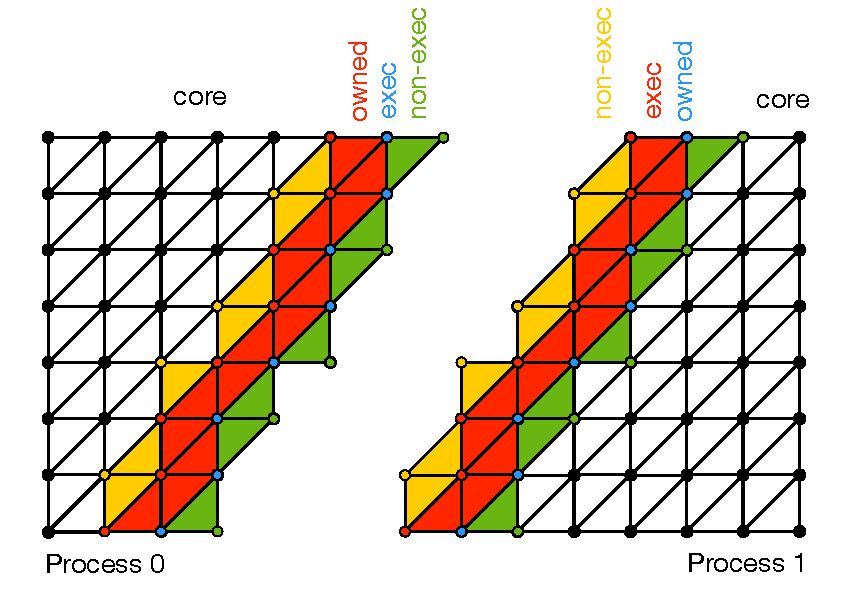
\includegraphics[scale=0.8]{background/figures/mpi_mesh}
\end{CenteredBox}
\caption{Distributed-memory parallelism in OP2 and PyOP2. Matching colors represent identical subsets of iterations. The image was inspired by an example in~\cite{florian-thesis}.}
\label{fig:bkg:sets-division}
\end{figure}

%The separation into four regions 

%In spite of a simple execution model, the implementation of distributed-memory parallelism requires a great deal of effort. 

\subsubsection{PyOP2 Features}
PyOP2 distinguishes itself from OP2 in a number of ways.

\begin{itemize}
\item An OP2 program is analyzed statically. A source-to-source compiler produces a legal C program, which can subsequently be compiled and executed. PyOP2, on the other hand, is implemented in Python, so code generation occurs at run-time; the generated C code applies a computational kernel over a set of elements. One problem with OP2 is that its source-to-source compiler is quite limited in the analysis of input programs. PyOP2 does not have this problem, because objects like sets, maps and parallel loops are constructed and inspected during the interpretation of the source program itself. This makes PyOP2 easily composable with other layers, as proven in the context of the Firedrake project. A hierarchy of ``software caches'' is however needed in PyOP2 to minimize the overhead due to redundant actions (e.g., generating code each time the same parallel loop is encountered).

\item Despite sharing relevant constructs (e.g., sets, maps), the PyOP2 domain specific language tends to be more compact and expressive than the OP2 counterpart. This is again a consequence of the run-time analysis.

\item PyOP2 supports global sparse matrices, basic linear algebra operations and mixed types (e.g., mixed sets), which are essential features for integration with a finite element framework. OP2 has none of these. 

\item OP2 completely handles distributed-memory parallelism, including partitioning and distribution of data structures as well as mesh renumbering for increased data locality. PyOP2, as explained in Section~\ref{sec:bkg:dmplex}, relies on an external software module, DMPlex, for these functionalities. DMPlex is much more versatile than OP2, and this plays a key role in performance optimization, as explained in Chapter~\ref{ch:sparsetiling}.
\end{itemize}



\subsection{Stencil Languages}
\label{sec:bkg:stencil-lang}

%Many computational methods, typically based upon finite difference or close variants, can then be described by means of stencils operating on $n$-dimensional structured meshes.

A stencil defines how to access a set of values associated with a mesh element (e.g., vertex, cell) and its neighboring elements. In the literature, the word ``stencil'' is often used to refer to the special case in which the access rule is an affine function. This is the case of computational methods based on structured meshes, such as the finite difference method. However, since this thesis focuses on unstructured meshes, we generalize this notion. We characterize a stencil as follows:

\begin{description}
\item[Stencils for structured meshes] Given an element $\boldsymbol{i}$ in the mesh, a stencil is a vector-valued function $f(\boldsymbol{i}) = [f_1(\boldsymbol{i}), f_2(\boldsymbol{i}), ..., f_n(\boldsymbol{i})]$ which retrieves the $n$ elements that need to be accessed when updating $\boldsymbol{i}$. A function $f_j$ is affine and usually takes the form $f_j(\boldsymbol{i}) = \boldsymbol{i}*h + o$, with $h, o \in \mathbb{N}$.
\item[Stencils for unstructured meshes] Given an element $\boldsymbol{i}$ in the mesh and an affine access function $g$, a stencil is a vector-valued operator $f(\boldsymbol{i}, g) = [f_1(\boldsymbol{i}, g), f_2(\boldsymbol{i}, g), ..., f_n(\boldsymbol{i}, g)]$ which retrieves the $n$ elements that need to be accessed when updating $\boldsymbol{i}$. A function $f_j$ is non-affine and usually takes the form $f_j(\boldsymbol{i}, g) = g(\boldsymbol{i})*h + o$, with $h, o \in \mathbb{N}$.
\end{description}

\subsubsection{Stencil Languages for Unstructured Meshes}
OP2 is an example of a language for implementing stencil-based computations on unstructured meshes. The maps in the OP2 language implement non-affine stencils. 

Yet another example of language for unstructured mesh stencils is Liszt \citep{lizst}. Like OP2, Liszt supports multiple architectures, including distributed-memory execution via MPI and GPUs. The language is less flexible than OP2's, though. Meshes are constructed by composing the abstract data types of the language, namely vertices, edges, faces and cells, and fields can only be associated with these types. This is on one hand helpful, as the stencils can automatically be inferred (assuming that the mesh topology does not change over time), but on the other hand it makes integration with a finite element framework difficult, or simply unnatural. Consider the case\footnote{The example was extracted from \cite{florian-thesis}} in which quadratic or higher-order basis functions on triangles are used. The degrees of freedom are associated with both vertices and edges. In OP2, this is naturally expressible by defining a map between cells and degrees of freedom, whereas in Liszt one needs to manage two different fields (one for the degrees of freedom on the vertices and the other for those on the edges). A computation in Liszt is expressed through sequences of {\em for-comprehensions} over mesh elements. The for-comprehensions can be arbitrarily nested. One of the key prerequisites is that each field in a for-comprehension nest has a fixed state, one among read, write, or increment (for local reductions). This allows the compiler to automatically perform useful actions such as scheduling transformations (e.g., by rearranging iterations in a for-comprehensions nest) and placement of MPI calls. The Liszt compiler derives data dependency information automatically, while OP2 relies on access descriptors. 

\subsubsection{Stencil Languages for Structured Meshes}
The field of domain specific languages for structured mesh computations has received a large number of contributions over the last decade. 

SBLOCK~\citep{sblock-cite} is a Python framework for expressing computations using structured stencils. The run-time support automatically generates low-level code for multi-node many-core architectures. Mint is a framework based on pragma directives targeting GPUs that has been used to accelerate a 3D earthquake simulation~\citep{mint-simulation-cite}. Other stencil languages relying on auto-tuning systems for increasing the performance of the generated code were presented in~\cite{zhang-mueller-cite,datta-cite,patus}. 

An interesting approach is adopted in Pochoir~\citep{pochoir}, in which a compiler translates the high-level specification into cache-oblivious algorithms for multi-core CPUs. Interestingly, an attempt at integrating this system with a higher-level domain-specific language for finite difference methods failed due to constraints on the programming interface~\citep{TJ-OPESCI}. 

A stencil language explicitly aiming for generation of highly-efficient vector code was presented in~\cite{stencil-compiler}.

In spite of a large research effort, it is however not clear whether and to what extent these languages have been adopted in production code. 


\section{Compilers and Libraries for Loop Optimization}
\label{sec:bkg:codeopt}
In this section, we review state-of-the-art compilers and libraries for loop optimization. This will provide the necessary background for the contributions presented in Chapters~\ref{ch:sparsetiling} and~\ref{ch:lowlevelopt}.

\subsection{Loop Reordering Transformations}
\label{sec:bkg:loop-transf}
The study of high level transformations for the optimization of loops in imperative languages dates back to the sixties. The initial focus was on techniques for improving data locality in loop nests; this was motivated by the observation that many programs spend a considerable fraction of time in executing these regions of code. A survey on the main results achieved between the sixties and the nineties was provided by~\cite{bacon-comp-transf}. Over the last twenty years, there has been a great deal of effort in trying to improve the effectiveness of loop transformations, as well as in developing tools for automating them. General-purpose compilers have become increasingly sophisticated (especially the {\em Intel} and {\em Cray} compilers), although they still often miss powerful optimization opportunities. This is usually a consequence of complex or unstructured codes for which the analysis is too difficult or the lack of domain information. Polyhedral compilers, discussed in Section~\ref{sec:bkg:poly}, are particularly effective in relatively simple affine loop nests, but there is no compelling evidence that analogous results could systematically be achieved in real-world applications.

A class of optimizations relevant for this thesis is the one based on the {\em reordering} of loop nest iterations. Well-known optimizations belonging to this class are:

\begin{description}
\item[Interchange] This transformation consists of exchanging the position of two loops in a nest. Possible objectives are exposing as innermost loop a vectorizable dimension or increasing data locality. 
\item[Reversal] When a loop is ``reversed'', the order in which its iterations are executed is flipped. For instance, the reverse of a loop iterating from $0$ to $n-1$ with unitary increment is a loop from $n-1$ to $0$ with unitary decrement. This transformation can enable other transformations or, under certain circumstances, eliminate the need for some temporary variables.
\item[Skewing] Loop skewing, sometimes also called ``time skewing'' or ``time tiling'', aims to improve data reuse and to expose parallelism in wave-front computations. In these computations, one or more arrays are updated at every loop iteration and the updates propagate like a wave over the subsequent iterations (e.g., \texttt{A[i][j] = f(A[i-1][j], A[i][j-1])}). We expand on loop skewing in Section~\ref{sec:bkg:tiling}.
\item[Fission] Sometimes also referred to as loop distribution, loop fission ``splits'' a loop into a sequence of loops. The new loops have the same iteration space as the original one, but include only a subset of statements. This may improve or even affect data locality in a loop accessing a significant number of datasets. Increase in loop overhead is a negative effect of the transformation.
\end{description}

Further, to this class of optimizations belong the two fundamental loop reordering transformations studied in Chapter~\ref{ch:sparsetiling} in the context of unstructured stencils:
\begin{description}
\item[Fusion] A sequence of loops can be fused, or ``merged'', to improve data locality and reduce loop overhead. In the simplest instance, all loops in a sequence have the same iteration space and, given $S_1$ a statement in a first loop and $S_2$ a statement in a subsequence loop, $S_2$ does not modify any data read by $S_1$. In such a case, applying loop fusion is straightforward. In general, however, loops can have different bounds and the data dependencies in a set of statements may be non-trivial. In these cases, loop fusion becomes more challenging, or simply not feasible. The loop fusion problem has been tackled formally by~\cite{fusion-complexity}.
\item[Tiling] Also known as {\em blocking}, loop tiling is probably one of the most studied and powerful transformations. Its main goal is improving data locality, although it is also sometimes used to extract parallelism. The basic idea is to ``chunk'' the iteration space of a loop nest into partitions of a given shape. This requires major changes to the loop nest structure, as shown in Listing~\ref{code:loop-tiling}. In this example, square-shaped tiles are executed with the objective of increasing data reuse along the \texttt{j} dimension. Depending on properties of the loop nest such as data dependency pattern and control flow, automating or even just implementing tiling may pose significant challenges. In particular, tiling a loop nest in presence of stencils is a non-trivial problem. Early work on this transformation was presented in~\cite{early-tile-cite-1} and~\cite{early-tile-cite-2}. More recent studies have tackled automation and effectiveness of the tiling algorithms, such as~\cite{pluto,plutoplus,loopy-final}. The impact of the tile shape has been investigated by~\cite{tile-shape-1} and~\cite{tile-shape-2}. 
\end{description}


\begin{algorithm}[t]
\scriptsize\ttfamily
\SetAlgorithmName{LISTING}{}

// Original implementation\\
~\\
\KwSty{for} i = 1 \KwSty{to} N, 1\\
~~\KwSty{for} j = 1 \KwSty{to} N, 1\\
~~~~\KwSty{for} k = 1 \KwSty{to} N, 1\\
~~~~~~C[i][j] += A[i][k]*B[k][j];\\

~\\
~\\
// Tiled implementation\\
~\\
\KwSty{for} i0 = 1 \KwSty{to} N, b\\
~~\KwSty{for} j0 = 1 \KwSty{to} N, b\\
~~~~\KwSty{for} k0 = 1 \KwSty{to} N, b\\
~~~~~~\KwSty{for} i = i0 \KwSty{to} \KwSty{min}(i0+b-1, N)\\
~~~~~~~~\KwSty{for} j = j0 \KwSty{to} \KwSty{min}(j0+b-1, N)\\
~~~~~~~~~~\KwSty{for} k = k0 \KwSty{to} \KwSty{min}(k0+b-1, N)\\
~~~~~~~~~~~~C[i][j] += A[i][k]*B[k][j];\\


\caption{Illustration of loop tiling in a classic matrix-matrix multiplication kernel\protect\footnotemark. The matrices are square of size $N \times N$. If $b$ is chosen small enough to fit some level of cache, data reuse can be achieved.}
\label{code:loop-tiling}
\end{algorithm}

\footnotetext{The example is partly extracted from \url{www.netlib.org/utk/papers/autoblock/node2.html}}

\subsection{Composing Loop Tiling and Loop Fusion}
\label{sec:bkg:tiling}
Reordering transformations can be composed for improving their effectiveness. A case of particular interest for this thesis is the composition of loop fusion and loop tiling, in which a sequence of loops is fused by grouping multiple blocks of iterations into tiles. Such a transformation can turn data reuse across consecutive loops into data locality, thus optimizing memory bandwidth and memory latency. Composing loop fusion and loop tiling is complicated; automation is even more challenging, especially depending on the kind of stencils that need to be supported.

In the domain of computational methods for approximating the solution of PDEs, the composition of loop fusion and loop tiling is often referred to as {\em time tiling}. In these codes, a sequence of loops over the spatial dimensions is repeatedly executed within a time loop; time tiling fuses the spatial loops by building tiles crossing the time dimension. Time tiling has extensively been studied for structured stencil codes~\citep{cohen-timetiling,ics-stencil-tiling,Zhou12,pluto}. It has instead received very limited attention in the context of unstructured stencil codes -- where it is also known as {\em sparse tiling}~\citep{ST-StroutLCPC2002} -- because of the complexity inherent in performing data dependence analysis. Prior to this thesis, sparse tiling had only been applied ``manually'' to individual benchmarks, through ``ad-hoc'' strategies. In Chapter~\ref{ch:sparsetiling}, the state-of-the-art is advanced by introducing:
\begin{itemize}
\item A technique for applying sparse tiling to {\it arbitrary} sequences of loops that are expressible with the {\em loop chain abstraction}~\citep{ST-KriegerHIPS2013}. This contribution was a joint effort with the authors in~\cite{st-paper}.
\item A system that automates this technique and enables execution on distributed-memory architectures.
\end{itemize}

With plain loop tiling (i.e., in the absence of loop fusion), a tile can be represented as a single block of iterations. This has been explained in the previous section and illustrated in Listing~\ref{code:loop-tiling}. Time and sparse tiling generalize this idea. The fused loops may either differ in iteration space or be characterized by non-trivial data dependencies. For constructing a legal scheduling, tiles need be assigned multiple blocks of iterations, one for each of the fused loops. To this purpose, there exist two different approaches:
\begin{description}
\item[Split tiling] Tiles are constructed such that all data dependencies are satisfied and are executed according to a partial ordering. Many split tiling schemes have been studied for structured stencil codes. These schemes, which take the name of the tile shape they end up producing (such as {\em hexagonal} or {\em diamond} tiling), differ in the achieved trade-off between parallelism and data locality. The geometrical shape of a tile can be visualized by plotting the fused iteration space and by grouping iterations based on the tile they belong to.
\item[Overlapped tiling] Different tiles share subsets of iterations. A shared iteration is ``owned'' by only one tile and is executed redundantly by the set of overlapping tiles. These tiles store intermediate values into ``ghost'' regions of memory. This approach removes the need for a partial execution ordering, at the price of redundant computation.
\end{description}
Some of these approaches have been reviewed in~\cite{survey-tile-shape}. In this thesis, we will employ a mixed split-overlapped sparse tiling scheme for unstructured stencil codes, suitable for execution on distributed-memory architectures.

% sparse tiling is a split scheme

\subsection{Automation via Static Analysis}
\label{sec:bkg:poly}
There are two alternatives for automating loop reordering transformations. Both of them rely on static analysis of source code:

\begin{description}
\item[Graph-based Representation] General-purpose compilers analyze the source code and produce an intermediate representation (IR) based on a graph-like data structure (e.g., the static single assignment form, or SSA, in the LLVM compiler). Some kind of data dependence analysis asserts the legality of a transformation, while cost models are used to predict its impact on performance. Some compilers can expose the cost models directly to the user by textual reports. Users have some form of control over the optimization process: pragma directives can be used to choose explicitly how to optimize a loop nest (e.g., to set a specific unroll factor or to enforce vectorization), while compiler parameters allow tuning global optimization heuristics. 
\item[Polyhedral Model] Several research compilers, and more recently also a fork of the LLVM compiler through a module called Polly~\citep{polly}, can introduce reordering transformations based on geometric representations of loop nests. To model a loop nest as a {\em polyhedron}, two conditions must be satisfied: (i) loop bounds as well as array indices must be affine expressions in the enclosing loop indices and (ii) pointer aliasing must be known at compile-time. These conditions are often necessary in the case of graph-based IRs too, although in a more relaxed fashion (e.g., the Intel compiler can vectorize, to some extent, non-affine loop nests). Polyhedral compilers target parallelism and data locality by composing {\em affine scheduling functions}. A schedule defines the order in which the statement instances of a loop nest are executed; a scheduling function can be applied to change the original order. Once the polyhedron is available, different scheduling functions can be compared and applied.
\end{description}

%A compiler performs data dependence analysis to determine the legality of a reordering transformation. In case a transformation is found legal, a cost model is used to predict its impact on the performance. If also the cost model provides positive feedback, the transformation is finally introduced by manipulating the IR. 

If, on one hand, general-purpose compilers using graph-based IRs have now reached an impressive level of sophistication (our experience with the Cray and Intel autovectorization systems is remarkably positive), there is still quite a lot of debate on the effectiveness of polyhedral compilers. One of the main reasons is the lack of evidence: the performance evaluation of state-of-the-art polyhedral compilers is typically conducted on simplistic benchmarks that do not reflect the complexity of real-world applications. We will expand on this matter in Section~\ref{sec:tiling:difficult}.

The fact that we focus on unstructured stencil codes, which render the loop nests non-affine, precludes the adoption of polyhedral compilers. Recently, there has been an effort in extending the polyhedral model to non-affine loops~\citep{sparse-poly-framework}, but it is far from clear whether this technology will ever be applicable in the real-world applications we are interested in.


\subsection{Automation via Dynamic Analysis}
\label{sec:bkg:ie}

If a stencil is unstructured, the memory access pattern is characterized by indirect accesses that can only be resolved at execution time. In such a case, loop reordering transformations can be enabled through inspector/executor strategies, as originally proposed by~\cite{ST-Saltz91}. Informally, an inspector is an additional piece of code that, at run-time, captures the data dependency pattern of an irregular loop nest into a suitable data structure. An executor is semantically equivalent to the original loop nest, but performs the iterations in a different order exploiting the information produced by the inspector. Examples of reordering transformations through inspector/executor schemes were provided by~\cite{ST-StroutPLDI03}. 

To automate a reordering transformation in the presence of unstructured stencils, a compiler replaces loops with suitable inspector/executor schemes. Prior to this thesis, no compilers were capable of introducing complex transformations such as sparse tiling.


%Space filling curves for unstructured meshes
%sparse tiling = loop fusion + loop tiling




\section{Domain-Specific Optimization}
\label{sec:bkg:dslopt}
%By targeting affine loop nests, polyhedral compilers are theoretically applicable in a wide range of programs, including computational methods for approximating the solution of PDEs, linear algebra routines, and image processing kernels. 
By restricting the attention to relatively narrow classes of programs, it is often possible to identify optimization opportunities that will be missed by general-purpose or polyhedral compilers. This is because, for instance, such optimizations rely on special mathematical properties of the problem being tackled. Most of the contributions in Chapters~\ref{ch:sparsetiling},~\ref{ch:optimality} and~\ref{ch:lowlevelopt} exploit this observation. In this section, we review some of the domain-specific optimization systems that inspired our work. 

\subsection{Tensor Contraction Engine}
\label{sec:bkg:tce}
The Tensor Contraction Engine (TCE) is a successful project that turns the mathematical structure of expensive computations in the field of quantum chemistry into powerful optimizations~\citep{TCE-url}. These codes need to execute long sequences of tensor contractions, or generalized matrix multiplications, which can easily result in teraflops of computation and terabytes of data for simultaneously storing huge dense matrices. The TCE provides a domain-specific language to express formulae in a mathematical style. The mathematical specification is transformed into low-level code while undergoing several optimization steps. Transformations aimed at reducing the operation count~\citep{TCE-2006,TCE-2009} and finding the best trade-off between redundant computation and data locality~\citep{TCE-2011}, as well as low-level optimization~\citep{TCE-2012} are applied in this framework. Many of these optimizations exploit the mathematical structure inherent in tensor contractions.

In Chapter~\ref{ch:optimality} we use a similar approach for optimizing the operation count of finite element operators -- we exploit the mathematical property that these operators are linear in test and trial functions to identify effective factorizations.


\subsection{Halide}
\cite{Halide} recently introduced Halide, a high level language for expressing image processing kernels. The run-time optimization system, which relies on auto-tuning to explore the transformation space, has been demonstrated to achieve a performance at least comparable to that of hand-written (and hand-optimized) codes, and in many cases to outperform them. Halide is a successful contribution to the landscape of domain-specific languages, as it is currently employed for development of production code by several companies\footnote{At least Google and Adobe have declared that some of their groups (more than 30 researchers and developers in total) are actively using Halide.}.

In Halide, an image processing pipeline is a sequence of interconnected stages. Each stage applies a numerical kernel -- usually a structured stencil -- to its input. Numerical kernels are pure functions applied over a 2D domain representing the image being processed. In realistic cases, an image processing pipeline can be quite complex and include even up to a hundred stages. What makes Halide powerful from the viewpoint of optimization is the fact that the schedules are decoupled from the numerical kernels. A schedule describes aspects like the iteration ordering and the trade-off between temporary values and redundant computation. These optimizations are fundamental in image processing pipelines and, as such, are treated as first-class citizens by Halide. Different schedules can be explored automatically or provided as user input.


\subsection{Spiral}
Spiral is a pioneering project on automated code generation starting from a high level specification of a mathematical problem~\citep{Pueschel:05}. The domain of interest is digital signal processing (DSP). Spiral generates highly optimized DSP algorithms, such as the discrete Fourier transform, and autonomously tunes them for the underlying platform. To achieve that, the mathematical specification of a DSP algorithm is first transformed according to a set of rewrite rules. The resulting formulae are translated into an intermediate language, which enables a set of optimizations, including explicit vectorization and parallelization. Finally, low level code is produced, compiled, executed and timed. The last phase provides feedback to the system so that increasingly optimized implementations can be generated. 

Spiral leverages the mathematical specification to apply powerful optimizations. The rewrite rules system itself is essential to simplify complex formulae. Another example is the loop fusion framework~\citep{spiral-fusion}, which exploits mathematical properties to detect loop fusion opportunities that would be missed by lower level compilers.


\subsection{Small-scale Linear Algebra}
In several fields, such as graphics, media processing and scientific computing, many operations can be cast as small-scale linear algebra operations. By small-scale we mean that the size of some of the involved tensors can be as small as a few units, and only occasionally exceed a few hundreds elements. Despite the small size, it is important to optimize these operations because they may be applied iteratively (e.g., in a time-stepping loop), thus accounting for a significant fraction of the overall execution time. 

Libraries for linear algebra are tuned for large-scale problems and they become inefficient when tensors are small. Novel approaches, mostly centred on auto-tuning, have been developed over the last decade. In the domain of scientific computing, it is worth mentioning the technique employed by the finite element code {\em nek5000}~\citep{nek5000-web-page} to optimize small matrix multiplications~\citep{nek5000}. A set of highly-optimized routines, each routine specialized for a particular size of the input problem, are generated and tuned for the underlying platform. At run-time, a dispatcher function picks one of such routines, based on the size of the input matrices. A higher level approach has recently been presented in~\cite{Spampinato:14}, in which the {\em LGen} language is used to write composite linear algebra operations. A set of rewrite rules and a transformation system deeply inspired by Spiral are used for optimization. Other libraries that are optimized for small-scale tensor operations include {\em LIBXSMM}~\citep{libxsmm} and {\em BLIS}~\citep{blis}.

The field of small-scale linear algebra optimization systems is interesting because some techniques could be used for low-level optimization of finite element local assembly, a topic treated by this thesis in Chapter~\ref{ch:lowlevelopt}.


\section{On the Terminology Adopted}
\label{sec:bkg:terminology}
Throughout the thesis we employ a standard terminology, very close to the one used in reference textbooks such as~\citep{patterson-book}. We here review a set of relevant keywords. This will especially be useful when discussing the performance achieved by the proposed optimizations.

%It may be useful to refer back to this section during the reading of the later chapters,  -- especially when analyzing the performance achieved by the proposed optimizations.


\subsection*{Compilers}

\begin{description}
\item[General-purpose compiler] With this term we generically refer to any open-source or commercial compilers capable of translating low level source code (e.g., Fortran, C, C++) into machine code. Examples are the GNU ({\em gcc}), Intel ({\em icc}), Cray and LLVM compilers. With ``general-purpose'' we aim to distinguish the aforementioned compilers from all other higher level compilers, such as those based on the polyhedral model or those used for translating domain specific languages.

\item[(Auto)vectorization] Vectorization is a well-known paradigm that generalizes computation on scalars to computation on vectors -- that is, arrays of contiguous elements. A single instruction, multiple data (SIMD) computation is one that employs vectorization to carry out a sequence of instructions. SIMD architectures, which are nowadays ubiquitous, emit vector code in two circumstances: (i) sections of a program are explicitly vectorized (e.g., through high level libraries, intrinsics instructions, or assembly code); (ii) a compiler transforms scalar code into vector code. The latter case is often referred to as autovectorization, since SIMD instructions are generated without user intervention. When possible and if demonstrated to be effective, autovectorization should be preferred over explicit vectorization for portability reasons. Autovectorization is typically applied to inner loops, although block vectorization~\citep{SLP-vect} is also supported by more advanced compilers (e.g., Intel's).

\end{description}


\subsection*{Performance and Cost Models}
\begin{description}

\item[(High) Memory pressure] This is often used to emphasize the fact that one or more levels of the memory hierarchy (e.g., RAM, caches, registers) are stressed by a relatively large number of load/store instructions. A high memory pressure is often responsible for performance degradation.

\item[Memory- and CPU-boundedness] A section of code can be either CPU-bound or memory-bound. In the former case, the performance achieved is limited by the operation throughput of the CPU; in the latter case, the memory bandwidth or the memory latency are the limiting factors. The loop reordering transformations reviewed in Section~\ref{sec:bkg:codeopt} tackle memory-boundedness; for example, both tiling and fusion aim to maximize the cache hit ratio, thus reducing latency and memory pressure. Many domain-specific optimizations, as discussed in Section~\ref{sec:bkg:dslopt}, target instead CPU-boundedness; for example, the Tensor Contraction Engine and Spiral manipulate mathematical formulae to reduce the operation count of the resulting kernels.

\item[Operational intensity and Roofline Model] This parameter defines the ratio of total operations to total data movement (bytes) between the DRAM and the cache hierarchy for a given section of code. The operational intensity, which ``{\it predicts the DRAM bandwidth needed by a kernel on a particular computer}``, is useful to derive {\em roofline plots}~\citep{roofline-cite}. A roofline plot is particularly helpful to study the computational behaviour of a program, since it provides an insightful means to understand what the performance bottleneck is and, therefore, what kind of optimization is most useful.

\item[Arithmetic intensity] Sometimes, the term {\em arithmetic intensity} is used in place of {\em operational intensity}. The differences are that only the fraction of arithmetic operations emitted, instead of all operations, is considered and that the total data movement is to be interpreted as between the CPU and the last level of cache.
\end{description}

\subsection*{Miscellanea}
\begin{description}

\item[Access function] An access function specifies how the elements of an array are accessed. Usually, these are functions of one or more loop indices. Access functions can be constant, affine or non-affine, as already shown in Section~\ref{sec:bkg:stencil-lang}.

\item[Local and global reductions] A reduction is a commutative and associative operation that is applied to a set of values to produce a scalar. For instance, the sum of a set of numbers is a reduction. In mesh-based computations, it is useful to distinguish between local and global reductions. A reduction is local if only applied to a (typically small) subset of mesh elements. A reduction is global if applied to an entire set of elements (e.g., a field associated with a set of degrees of freedom), thus introducing a global synchronization point in the computation. 

\item[Communication] A communication indicates a generic form of interaction between two or more entities. The most obvious case is when two processes on two different cores communicate explicitly via message passing; if the cores are on the same node the communication occurs via memory, whereas if they are on different nodes both the network and the memory are needed. However, the term can also be used in more general scenarios. We can say, for instance, that two tiles in a blocked iteration space communicate if their execution needs be synchronized. Intuitive terms like {\em communication-avoiding} or {\em communication-computation overlap} are often used to classify optimizations that aim to minimize communication.

\item[Real-world applications] Throughout the thesis we emphasize the use of realistic applications, as opposed to simplistic benchmarks, to evaluate the impact of the introduced optimizations. By ``real-world'' we mean that an application is based upon real-life equations, numerical methods, and datasets. By using real-world applications, we aim to provide compelling evidence about the effectiveness and the actual applicability of our contributions.
\end{description}

